\section{Techniques}

This section gives an overview of different techniques used in our crawler. We first show how we integrated a headless web browser into the harvesting process to support blogs that use JavaScript to display page content. The overall software architecture will then be discussed, introducing the Scrapy framework and the enrichments we implemented for our specific use case. Finally we will talk about deployement to scalable, fault resilient distributed architecture.


%%%%%%%%%%%%%%%%%%%%%%%%%%%%%%%%%
\subsection{JavaScript rendering}
% Introduction
JavaScript is a widely used language for client-side web scripting. While some applications simply use it for aesthetics (menus, animations...), an increasing number of websites use JavaScript to download and display content. In such cases, traditional HTML based crawled do not see web pages as they would be presented to a human visitor and might therefore be obsolete for data extraction.

% Motivation
In our experiments crawling the blog sphere, we encountered several blogs where data was missed because of the lack of JavaScript interpretation. The most frequent cases where blogs using the Disqus \cite{disqus2013} and LiveFyre \cite{livefyre2013} comment hosting services. These tools are very handy to setup for web-masters because the entire comments infrastructure is externalized and the setup essential comes down to including a JavaScript snippet in each target page. Both of these services heavily rely on JavaScript to download and display the comments, even providing functionalities such as real-time updates for edits and newly written comments. Less commonly, some blogs are fully rendered using JavaScript. When loading such website, the web browser will not receive the page content as an HTML file, but will instead have execute JavaScript code to download and display the page content. One example can be found on the Blogger platforms which provides as one of its default templates the \emph{Dynamic Views} which use this mechanism \cite{antinharasymiv2011}.

% The solution
To support blogs with JavaScript generated content, we embed a full web browser into the crawler. After considering multiple option, we opted for PhantomJS \cite{phantomjs2013}, a headless web browser with great performances and scripting capabilities. The JavaScript rendering is done as the very first step of web page processing. Extracting blog post content, comments or images therefore works equally well on both blogs with JavaScript generated content and traditional HTML-only blogs.

% Click click scripting
When the number of comments on one page exceeds a certain threshold, both Disqus and LiveFyre only load a subset of them and end the stream of comments with a \emph{Show More Comments} buttons. As part of the page loading process, we instruct PhantomJS to repeatedly click on these buttons until all comments are loaded. Paths to Disqus and LiveFyre \emph{show more} buttons were manually obtained and are the only non-generic element of the extraction stack which will require human intervention to maintain and extend to other commenting platforms.


%%%%%%%%%%%%%%%%%%%%%%%%%
\subsection{Architecture}

\begin{figure}
  \capstart
  \centering
  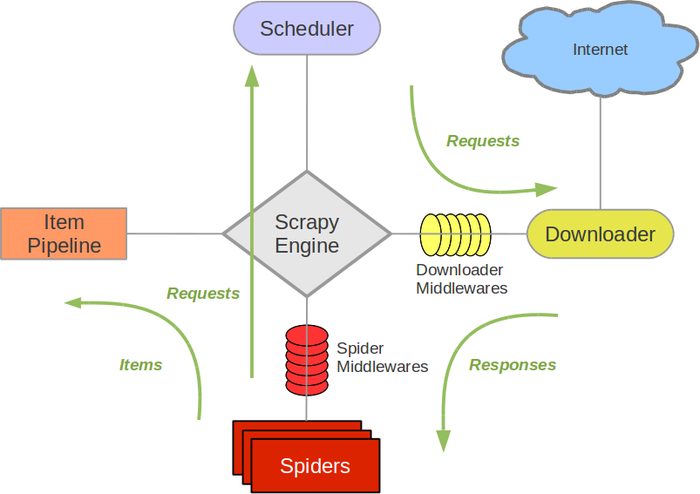
\includegraphics[width=0.47\textwidth]{img/scrapy_architecture.png}
  \caption{Overview of the crawler architecture.\\(Credit: Pablo Hoffman, Daniel Graña, \cite{scrapy2013})}
  \label{architecture}
\end{figure}

Our crawler is built on top of Scrapy\cite{scrapy2013}, an open source Python framework for web crawling. Scrapy provide an elegant and modular architecture illustrated in Figure~\ref{architecture}. Several components can be plugged in Scrapy core infrastructure: \emph{Spiders}, \emph{Item Pipelines}, \emph{Downloader Middlewares} and \emph{Spider Middlewares}; each allowing to implement a different type of functionalities.

Our use case has two types of spiders: \emph{NewCrawl} and \emph{UpdateCrawl}, which respectively implement the logic to crawl a new blog and to get updates from a previously crawled blog. After downloading its HTML\TODO{rephrase!}, a web page is packed into an \emph{Item} and sent through the following pipeline of operation:
\begin{enumerate}[noitemsep]
  \item Render JavaScript
  \item Extract content
  \item Extract comments
  \item Download medias
  \item Propagate resulting records to the Invenio back-end
\end{enumerate}
This pipeline design, often called \emph{pipes and filters pattern} \cite[Chapter Messaging Systems]{hohpe2003}, provides great modularity. Indeed, disabeling JavaScript rendering or plugging in an alternative back-end can be done by editing a single line of code.


%%%%%%%%%%%%%%%%%%%%%%%%%%%%%
\subsection{Enriching Scrapy}
% Into, blog post identification
In order to identify web pages as blog posts, our implementation enriches Scrapy with two components to narrow the extraction process to the subsets of blog pages holding blog posts: \emph{blog post identification} and \emph{download priority heuristic}. Given an entry point to a website, the default Scrapy behavior allows to look over all pages of the same domain in a \emph{last-in-first-out} manner. The \emph{blog post identification} function is able to identify from an URL whether or not the corresponding page is a blog post. Internally, this function uses a regular expression constructed for each blog from it's web feed entries. These constitute the only set of known blog post URLs, and can therefore be used to identify the structure of blog post URLs. This simple approach requires that blogs use the same pattern for all posts (or false negative will occur) which has to be distinct for non-post pages (or false positive will occur). In practice this assumption held for all blog platforms we encountered during the developments and seems to be a common practice among web developer.

% download priority heuristic
In order to efficiently deal with blogs with a large number of non-blog-post pages, this blog post identification mechanism is not sufficient. Indeed, after all pages identified as blog post are processed, the crawler needs to download non-blog post pages to search for additional blog posts. To replace the naive random walk, depth first search or breadth first search web site traversals, we use a priority queue where new URL priorities are determined using a simple machine learning algorithm. Given an URL, the machine learning system does an estimation on the number of links to blog post the corresponding page will contain. This estimated number of links are then used as a \emph{download priorities} to decide the best URL to visite next. Each time a page is effectively downloaded, the actual number of blog post links it contains is computed and passed to the machine learning system as training data that will then be taken into account during future predictions. This mechanism has shown to be indispensable for blogs hosting on the single domain a large number of non-blog web pages, such as a forum or a wiki.

Due to space constraints, more precise description and evaluation of these two components where not included in this paper.
\TODO{Again these things are great and you should write a lot more, instead of explaining Javascript rendering so much in 4.1  (it is trivial compared to these nice algorithms).}

%%%%%%%%%%%%%%%%%%%%%%%%
\subsection{Scalability}
\TODO{merge with 4.3, remove all the usless things. I believe that scalability should be removed from here and included in future work in the end.

Also, everyone knows what scalability is and we don't have a lot of space as we said earlier :)
The Reactive manifesto is not necessary...}
When aiming to work with a large number of inputs, it is crucial to build every layer of the system with scalability in mind. Citing the Reactive Manifesto \cite{thereactivemanifesto2013}:

\begin{quoting}
  If one of these layers does not participate—making blocking calls to the database, relying on shared mutable state, calling out to expensive synchronous operations—then the whole pipeline stalls and users will suffer through increased latency and reduced scalability.
\end{quoting}

At the time of writing we did not had the chance to work on the deployment of the BlogForever project on a distributed environment. However, the BlogForever crawler, and in particular the two core procedures \emph{NewCrawl} and \emph{UpdateCrawl}, where designed to be usable as part of an event-driven, scalable and fault resilient distributed system.

\Anotecontent{noteC}{Blogs that do not provide a global comment feed need a special handling. If comment feeds are attached to each blog post, periodically checking for comment updates might be done with a reasonable cost. However, in the worst case where no comment feeds are provided, the only solution is to periodically do a full crawl of the blog to capture new comments.}

Scalability and fault resilience are induced by the fact that both \emph{NewCrawl} and \emph{UpdateCrawl} are from a high level viewpoint stateless entities. \emph{NewCrawl} can be seen as a function, which takes as input the URL of a blog and returns structured records for blog posts, comments and medias. Similarly, \emph{UpdateCrawl} takes as inputs the URL of blog\Anote{noteC} and a time, and returns records of objects that where emitted after the given time. The absence of state implies that in a distributed setup, crawler instances could be removed, added, and used interchangeably.

Regarding the asynchronous architecture, Scrapy is build upon Twisted\cite{twisted2013}, an event-driven networking framework for Python. Scrapy also provides a built-in service to start spiders with an HTTP JSON API. With these tools in hand, the only component to implement in order to achieve a scalable and fault resilient distributed crawling system is an entity to keep track of available crawlers and does appropriate load balancing between them.
